%======================= PREAMBOLO DICHIARAZIONI INIZIALI===============%
\documentclass[10pt,oneside,a4paper]{article}

\usepackage[latin1]{inputenc} 
\usepackage[italian]{babel}
\usepackage{siunitx} %Inserisce automaticamente i dati con le unità di misura correttamente formattate del SI (utilizzo: \SI{0.82}{m^2}, in generale \SI{misura con il punto decimale}{unità di misura})
\sisetup{output-decimal-marker = {.}, separate-uncertainty = true, input-uncertainty-signs = \pm, detect-weight=true, detect-family=true} %per usare SI con il punto decimale
\usepackage{listings} %Per citare codice informatico formattandolo correttamente
\usepackage{amsmath}
\usepackage{graphicx}
\usepackage{geometry}
\usepackage{epigraph}
\usepackage{booktabs}	%tabelle migliorate
\usepackage{tablefootnote}	%note a piè di pagina in tabella
\usepackage{threeparttable} %tabella con note a piè di tabella
\usepackage{caption}	%descrizione per figure
\captionsetup{tableposition=top,figureposition=bottom,font=small} %setup descrizione
\usepackage{float}
\usepackage{esvect} %vettori
\usepackage{longtable} %tabelle lunghe


\setcounter{section}{-1}

%========= PRIMA PAGINA ===========%
\title{\textsc{Misura dell'accelerazione di gravità attraverso lo studio del moto di un carrello su di un piano inclinato }}
\author{\small{G. Galbato Muscio} \and \small{L. Gravina} \and \small{L. Graziotto} \and \small{M. Rescigno}}
\date{}

\begin{document}
	\begin{figure}
		\centering
		\includegraphics[scale=0.5, trim={2.8cm 8.9cm 0 9cm}, clip]{logo.png}
	\end{figure}
	\maketitle
	\begin{center} 
		\fbox{{\fontsize{12pt}{8mm}\textsc{Gruppo B2.3}}} \\
		\vspace{1cm}
		\begin{tabular}{ccc}
			Esperienza di laboratorio && Consegna della relazione \\
			\emph{\small{20 aprile 2017}} && \emph{\small{2 maggio 2017}} \\
		\end{tabular} 
		
		\vspace{0.5cm}
		
	\end{center}
\hrule
\vspace{0.5cm}
\begin{abstract}
	Studiando dal punto di vista cinematico il moto di un carrello lungo un piano inclinato scabro, diamo diverse stime dell'accelerazione di gravità $g$ e del coeficiente di attrito dinamico $\mu_d$.
\end{abstract}
\newpage
\tableofcontents %Indice
\listoftables %Indice delle tabelle
\listoffigures %Indice dei grafici
\pagebreak
\section{Convenzioni e formule}
In questa relazione verranno usate le seguenti convenzioni:
\begin{enumerate}
	\item sarà usato il punto [ $.$ ] come separatore decimale;
	\item l'approssimazione decimale della cifra $5$ sarà fatta per eccesso;
	\item al fine di migliorare la qualità dell'elaborazione dei dati, ogni grafico/istogramma prodotto a mano su carta millimetrata sarà riportato insieme al suo equivalente prodotto attraverso un software di analisi dati\footnote{In questo contesto i dati sono stati elaborati con il software di analisi \emph{R}.};
	\item al fine di snellire la relazione e migliorarne la leggibilità, riporteremo nel corpo del documento solamente le tabelle riepilogative e dedicheremo un'appendice finale alle tabelle contenenti tutte le singole misure e i singoli risultati; data la mole di misure effettuate con il sonar spesso saranno riportate solo le sintesi dei dati.
\end{enumerate}
Inoltre, si farà riferimento alle seguenti formule:
\begin{enumerate}
	\item media 
	\begin{equation}\label{eq:media}
	\bar{x} = \frac{1}{N}\sum_{i=1}^Nx_i;
	\end{equation}
	\item varianza
	\begin{equation}\label{eq:varianza}
	\sigma^2 = \frac{1}{N}\sum_{i=1}^N(x_i-\bar{x})^2;
	\end{equation}
	\item deviazione standard
	\begin{equation}\label{eq:deviazione}
	\sigma = \sqrt{\sigma^2}.
	\end{equation}	
\end{enumerate}

%===============SCOPO E DESCRIZIONE DELL'ESPERIENZA==============%
\section{Scopo e descrizione dell'esperienza}
\label{sec:description}
Un carrello che si muove lungo un piano inclinato di un angolo $\theta$ rispetto all'orizzontale è soggetto a diverse forze. Proiettando tali forze lungo un asse parallelo e uno perpendicolare allo spostamento, le tre componenti che intervengono sono:
\begin{itemize}
	\item la forza peso che accelera il carrello
		\begin{equation}\label{eq:forzapeso}
 			 F_p=m g \sin\theta;
		\end{equation} 
   	\item la reazione vincolare del piano, che bilancia componente perpendicolare della forza peso 			
	    \begin{equation}\label{eq:reazionevincolare}
			N=mg \cos \theta;
		\end{equation}
	\item la forza di attrito dinamico tra il carrello e il piano inclinato, con verso opposto al moto e che decelera il carrello
		\begin{equation}\label{eq:forzaattrito}
			F_a=N\mu_d.
		\end{equation}
\end{itemize}
Dallo studio di queste forze sappiamo quindi che l'accelerazione totale del carrello è data da: 
\begin{equation}\label{eq:accelerazionetot}
	a_x=g(\sin\theta \pm \mu_d \cos\theta)
\end{equation}
dove il segno dipende dalla direzione dell'accelerazione (negativo nel caso discendente, altrimenti positivo). Nel caso di piccoli angoli ($\theta \le \SI{0.18}{rad}$) si possono approssimare:
\begin{equation}\label{eq:approssimazione}
	\sin\theta \approx \theta ;\qquad  \cos\theta \approx 1 \notag
\end{equation}
per cui la formula (\ref{eq:accelerazionetot}) per l'accelerazione totale diventa:
\begin{equation}\label{eq:accelerazionepiccoliangoli}
	a_x=g(\theta \pm \mu_d).
\end{equation}

In questa esperienza, dopo aver calibrato lo strumento per misure di posizione, daremo diverse stime di $\mu_d$ e di $g$ ottenute con pi� modalit�:

\begin{enumerate}
	\item misura del prodotto $g \cdot \mu_d$ con il piano in orizzontale, imprimendo una velocit� iniziale;
	\item misura di $g$ con un angolo fisso specifico;
	\item misura simultanea di $g$ e $\mu_d$ variando l'angolo di inclinazione;
	\item misura di $g$ ottenuta misurando tutto il moto sia nel tratto discendente che in quello ascendente.
\end{enumerate}
	
%================APPARATO SPERIMENTALE======================%		
\section{Apparato Sperimentale}
	
\subsection{Strumenti}
\label{subsec:strumenti}
\begin{itemize}
	\item Guida inclinata lunga circa due metri con scala graduata [divisione: \SI{1}{mm}, incertezza:];
	\item sonar in grado di misurare la distanza del carrello a tempi diversi [frequenza: \SI{20}{Hz}];
	\item software \emph{Data Studio} per raccogliere ed elaborare in modo preliminare le misure del sonar;
	\item squadra [divisione: \SI{1}{mm}, incertezza:];
	\item carrello;
	\item livella digitale [digit: \SI{1}{�}].
\end{itemize}

%==============SEQUENZA OPERAZIONI SPERIMENTALI============%
\section{Sequenza Operazioni Sperimentali.}

\subsection{Verifica degli strumenti.}
\label{subsec:verifica}
La guida risultava inclinata di circa \SI{-1}{�} quando i piedi erano completamente abbassati, la causa principale � attribuibile ad un'inclinazione della pavimentazione che, misurata, risultava anch'essa di circa \SI{-1}{�}. %, l'errore è stato corretto ottenendo così un piano orizzontale necessario per lo svolgimento delle prime misurazioni.
Oltretutto, la guida non era perfettamente piana bens� leggermente a catenaria, infossata nel centro (probabilmente a causa di un'assenza di supporti intermedi); non è stato possibile risolvere l'errore (si sarebbe dovuta cambiare la struttura della guida).
Il sonar è stato invece calibrato seguendo le modalit� indicate, come meglio approfondito nella sezione~\ref{subsec:Calibrazione}.

L'attrito tra il carrello e la guida era poco efficace, questo ha reso evidenti i difetti di costruzione della guida stessa sul moto del carrello.

Il software \emph{Data Studio}, necessario per interagire con il sonar, permette di scegliere arbitrariamente il numero di cifre significative con le quali memorizzare i dati, per cui l'ampiezza del digit non è ben definita: assumiamo come incertezza sulle misure di posizione esclusivamente quella di tipo \textbf{A}.

%================ CALIBRAZIONE ==================%
\subsection{Calibrazione delle misure di distanza}
\label{subsec:Calibrazione}
Lo strumento utilizzato per registrare le misure di posizione (sonar) deve essere calibrato: esso è tendenzialmente soggetto ad errori di offset e di scala (la velocità del suono dipende dai fattori ambientali). Per quanto detto nella sezione \ref{sec:description} la posizione del carrello ha un'importanza solo relativa: interessandoci della sua accelerazione e non della sua posizione assoluta (equazione \ref{eq:accelerazionepiccoliangoli}), l'offset non disturba le nostre misure indirette e l'unico parametro di calibrazione significativo è quello di scala; per misurare tale coefficiente è necessario posizionare il carrello sulla guida orizzontale e confrontare in un grafico le distanze misurate con il sonar e quelle di riferimento misurate con la scala millimetrata fissata alla guida. Dal grafico è possibile estrapolare la retta di calibrazione, la quale è descritta da un'equazione del tipo:
\begin{equation}\label{eq:rettacalibrazione}
	x_{r}=\alpha x_{m} + \beta
\end{equation}
dove $x_r$ è la distanza di riferimento e $x_m$ quella misurata, $\alpha$ � il coefficiente di scala e $\beta$ l'offset. Le misure sono state prese lasciando il sonar attivo per circa 10 secondi ad ogni misura, per un totale quindi di 200 (\SI{20}{Hz} $\cdot$ \SI{10}{s}) misure per posizione; sul grafico \ref{fig:calibrazione} sono stati riportati i valori medi per ogni distanza con la relativa incertezza $( \delta = \sigma / \sqrt{N})$, le misure sono sintetizzate nella tabella \ref{tab:calibrazione}. Estrapolando i parametri direttori della retta, risultano:
\begin{equation}\label{eq:parametri_calibrazione}
	\alpha = \SI{ 1.0361 \pm 0.0029}{}, \qquad \beta = \SI{ -0.351 \pm 0.0029}{m}, %Mettere i valori effettivi
\end{equation}
dove le incertezze sono state prodotte insieme ai parametri dal software $R$ con il metodo dei minimi quadrati.

\begin{table}
\caption{Misure di calibrazione}
\label{tab:calibrazione}
\centering
\begin{tabular}{c|cc}
\hline
$x_r [\SI{}{m}]$ & $x_m [\SI{}{m}]$ & $\delta$ [\SI{}{m}] \\
$\pm$ 0.00015 && \\
\hline
0.50000 & 0.52084 & 0.00012 \\
0.60000 & 0.61273 & 0.00003 \\
0.70000 & 0.70871 & 0.00008 \\
0.80000 & 0.80446 & 0.00002 \\
0.90000 & 0.89897 & 0.00007 \\
1.00000 & 0.99997 & 0.00001 \\
1.10000 & 1.09359 & 0.00008 \\
1.20000 & 1.19130 & 0.00005 \\
1.30000 & 1.29049 & 0.00005 \\
1.40000 & 1.38738 & 0.00002 \\
\hline
\end{tabular}
\end{table}

%=============== MISURA DI G-Mu==========%
\subsection{Misura di $g\mu_d$.}
Per ricavare una prima stima del prodotto del coefficiente di attrito dinamico $\mu_d$ per l'accelerazione di gravit� $g$ la guida viene posizionata orizzontalmente, verificando che il carrello, in assenza di stimoli esterni, rimanga in quiete. Il carrello viene poi messo in moto imprimendo un impulso che fornisce una velocit� iniziale dell'ordine di \SI{0.2}{m/s}.
Realizzando $5$ raccolte di dati otteniamo diverse stime della decelerazione del carrello dovute all'attrito. Infatti: 
\begin{equation}\label{eq:accelerazione1}
	\alpha a=-g\mu_d
\end{equation}
dove con $\alpha$ indichiamo il coefficente di calibrazione stimato nella prima fase dell'esperienza. \newline
Riportiamo nella tabella \ref{tab:medieacc} i valori delle medie di ciascuna raccolta con le rispettive deviazioni standard e incertezze sulle medie.
\begin{table}
	\caption{Medie delle 5 raccolte}
	\label{tab:medieacc}
	\centering
	\begin{tabular}{ccc}
		\hline
	    $ a $ & $ \sigma $ & $\sigma/\sqrt{N}$ \\
		\hline
		 -0.040 & 0.082 & 0.009 \\
		 -0.043 & 0.084 & 0.010 \\
		 -0.043 & 0.084 & 0.010 \\
		 -0.045 & 0.092 & 0.010 \\
		 -0.040 & 0.120 & 0.014 \\
		\hline
	\end{tabular}
\end{table}

Le distrinuzioni ottenute sono tra di loro compatibili in quanto differiscono al massimo per una $\sigma$. Con
\begin{equation}\label{eq:duesigma}
\sigma = \sqrt{\sigma_1^2 +\sigma_4^2} = \SI{0.12}{m/s^2}
\end{equation}
Dove con $\sigma_1$ indichiamo la deviazione standard della prima raccolta e con $\sigma_4$ la deviazione standard della quarta raccolta. Avendo verificato la compatibilit� delle 5 raccolte, la successiva analisi sar� svolta sulla totalità dei dati. \newline
L'istogramma rappresenta la distribuzione delle accelerazioni, ad una prima analisi risulta chiaramente incompatibile con un modello gaussiano in quanto agli estremi presenta dei raggruppamenti molto discostanti dai valori centrali. Queste anomalie, probabilmente legate a errori del sonar nella misura o a errori nel calcolo delle accelerazioni, possono essere eliminate permettendoci di ottenere una stima pi� precisa. Tali misure infatti non modificano significativamente la media ma influenzano la deviazione standard e ci conducono ad una sovrastima dell'errore statistico. 
Per provare che questi valori non rappresentano le code della distribuzione e sono incompatibili con il modello che ci aspettiamo, calcoliamo la probabilit� che, data una gaussiana di media (\SI{-0.046}{m/s^2}) e deviazione standard (\SI{0.048}{m/s^2} fornite dall'analisi di valori centrali, si verifichino tali eventi. Utilizzando la funzione \emph{"pnorm"} di \emph{R}, determiniamo che la probabilit� di ottenere un evento con valore maggiore di $0.2$ e minore di $-0.2$ è $2.0\cdot10^-3$. Ci aspetteremmo quindi $2.0\cdot10^-3\times N_{eventi} \approx 0.06$ eventi, da confrontare con i 33 effettivamente trovati ed eliminati dall'analisi successiva. L'istogramma in figura \ref{fig:istogramma_gmu} riporta blu i dati coerenti e in grigio quelli anomali che sono stati scartati.

\begin{figure}[h]
\centering
\caption{Istogramma delle accelerazioni ad angolo nullo}
\label{fig:istogramma_gmu}
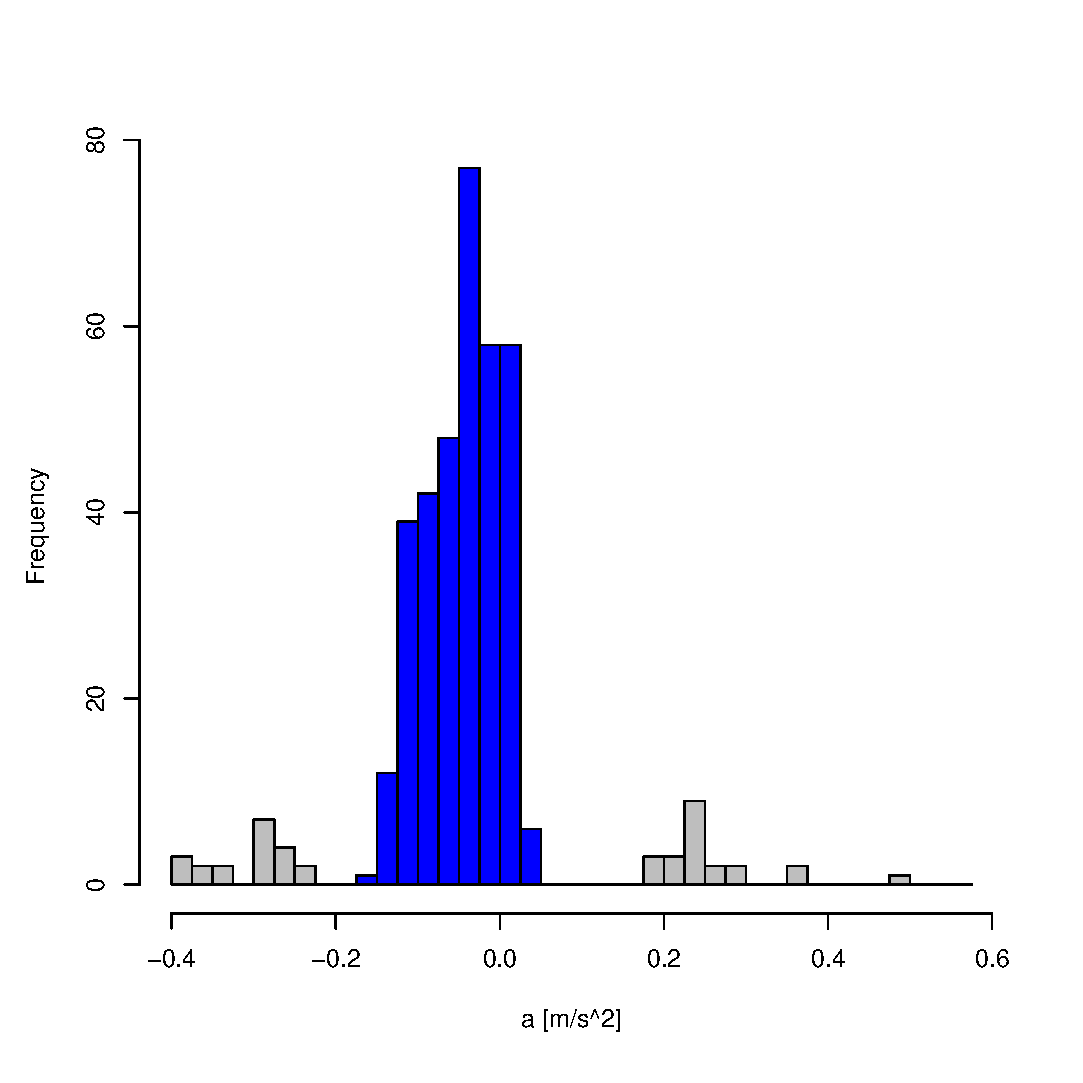
\includegraphics[scale=0.7]{istogramma.eps}
\end{figure}

La stima di $g\mu_d$ sar� quindi data dall'equazione \ref{eq:accelerazione1}, dove l'accelerazione media � ottenuta dai dati selezionati. L'errore da associare a tale misura � dato dalla propagazione delle incertezze su una forma monomia. Poich� la posizione orizzontale del carrello non è stata ottenuta misurando un angolo nullo, bens� verificando che il carrello fosse in quiete, non � necessario propagare l'incertezza sull'angolo. Il coefficiente di correlazione e l'accelerazione sono invece affette da un incertezza, per cui:
\begin{equation}\label{eq:incertezzarelativa}
\sigma_{g\mu_d} = g\mu_d\sqrt{\biggl(\frac{\sigma_\alpha}{\alpha}\biggl)^2+\biggl(\frac{\sigma_a}{a}\biggl)^2}
\end{equation}
Dove $\sigma_\alpha$ è l'incertezza sul coefficiente di calibrazione calcolata nel paragrafo mentre $\sigma_a$ � l'incertezza sulla media ed� quindi data dalla deviazione standard sul numero di misure. 
La migliore stima di $g\mu_d$ è quindi:
\begin{equation}
\boxed{\bf{g\mu_d= 0.046\pm }}
\end{equation}


%=================MISURA G ANGOLO SPECIFICO=============%
\subsection{misura dell'accelerazione di gravità con la misura dell'accelerazione ad un angolo specifico.}
Posizionando la guida inclinata ad un angolo $\theta$ abbstanza grande, in modo da ottenere una maggiore precisione, sono state relaizzate, sempre grazie al programma Data Studio, numerose stime (10 misurazioni da 10 secondi) dell'accelerazione mantenendo l'angolo $\theta$ fisso. Combinando i risultati ottenuti con le stime precedenti di $g\mu_d$ è possibile ottenere una stima delL'accelerazione di gravità $g$. 


%=============== ANGOLO VARIABILE========%
\subsection{Determinazione simultanea dell'accelerazione di gravità e del coeficiente di attrito variando l'angolo del piano inclinato.}
Variado l'angolo di inclinazione del piano, effettuiamo una misura di posizione da $10$ secondi per ogni angolo scelto. Facendo un grafico dell'accelerazione in funzione dell'angolo di inclinazione è possibile estrarre l'accelerazione di gravità dal coeficente angolare della retta che meglio approssima i punti. 



%============ SU E GIU' ========%
\subsection{Determinazione dell'accelerazione di gravità dalla differenza dell'accelerazione nel tratto discendente e quella nel tratto ascendente.}
Nell'ultima misurazione invece, tenendo l'angolo fisso a circa $0.05$ rad è stata misurata l'accelerazione sia nel tratto ascendente che discendente fino alla fine del moto del carrello. Dalla differenza delle due accelerazioni possiamo realizzare una stima di $g$
	\begin{equation}
	ax_x1= g(\theta + \mu_d) 
	\end{equation} (ascendente)\newline
	\begin{equation}
	a_x = g(\theta - \mu_d)
	\end{equation} (discendente)
Da cui facendo la differenza delle due accelerazioni otteniamo una stima di $g$.





%==== CONSIDERAZIONI FINALI =========%
\section{Considerazioni finali.}




\newpage
\section{Appendice: tabelle e grafici}



\end{document}
